% NB: use pdflatex to compile NOT pdftex.  Also make sure youngtab is
% there...

% converting eps graphics to pdf with ps2pdf generates way too much
% whitespace in the resulting pdf, so crop with pdfcrop
% cf. http://www.cora.nwra.com/~stockwel/rgspages/pdftips/pdftips.shtml




\documentclass[12pt,aspectratio=169]{beamer}
%\usetheme[everytitleformat=uppercase]{m}
\usetheme[everytitleformat=regular,color/block=transparent]{m}
\usepackage[absolute,overlay]{textpos}
\usepackage{booktabs}

\usepackage{graphbox} %loads graphicx package

\usepackage{pbox}

\usepackage{adjustbox}

\usepackage[utf8]{inputenc}


\usepackage[scale=2]{ccicons}


\usepackage[official]{eurosym}



%use this to add space between rows
\newcommand{\ra}[1]{\renewcommand{\arraystretch}{#1}}

% for sources http://tex.stackexchange.com/questions/48473/best-way-to-give-sources-of-images-used-in-a-beamer-presentation

\setbeamercolor{framesource}{fg=gray}
\setbeamerfont{framesource}{size=\tiny}


\newcommand{\source}[1]{\begin{textblock*}{5cm}(9.7cm,8.3cm)
    \begin{beamercolorbox}[ht=0.5cm,right]{framesource}
        \usebeamerfont{framesource}\usebeamercolor[fg]{framesource} Source: {#1}
    \end{beamercolorbox}
\end{textblock*}}

\usepackage{hyperref}


%\usepackage[pdftex]{graphicx}


\graphicspath{{graphics/}}

\DeclareGraphicsExtensions{.pdf,.jpeg,.png,.jpg}



\let\olditem\item
\renewcommand{\item}{%
\olditem\vspace{5pt}}

\title{
}
%\subtitle{---}
\author{
  \emph{Tom Brown, Robbie Morrison, The Open Energy Modelling Initiative Community}
}

\date{\vspace{0.5cm}Open Power System Data 4th Workshop, DIW Berlin, 10th July 2017}


\titlegraphic{%
  \vspace{0.7cm}
  % left bottom right top
  
\includegraphics[width=12.5cm]{openmod-logo-vector}

}



\begin{document}

\maketitle

\begin{frame}
  \frametitle{openmod: overview}

\begin{itemize}
  \item \alert{grass roots community} of open energy modellers from universities
  and research institutions
  \item participants mainly from Europe, but also from Africa, America,
    and Australia
  \item first meeting Berlin 18–19 September 2014 as an off-shoot of
    strommarkttreffen (some founding members started OPSD)
  \item promoting \alert{open code}, \alert{open data} and \alert{open science}
\end{itemize}
\end{frame}


\begin{frame}
  \frametitle{what is open modelling?}

  \alert{Open} refers to model source code that can be studied,
  changed and improved as well as freely available energy system data. The \alert{whole pipeline} should be open:

  \centering
  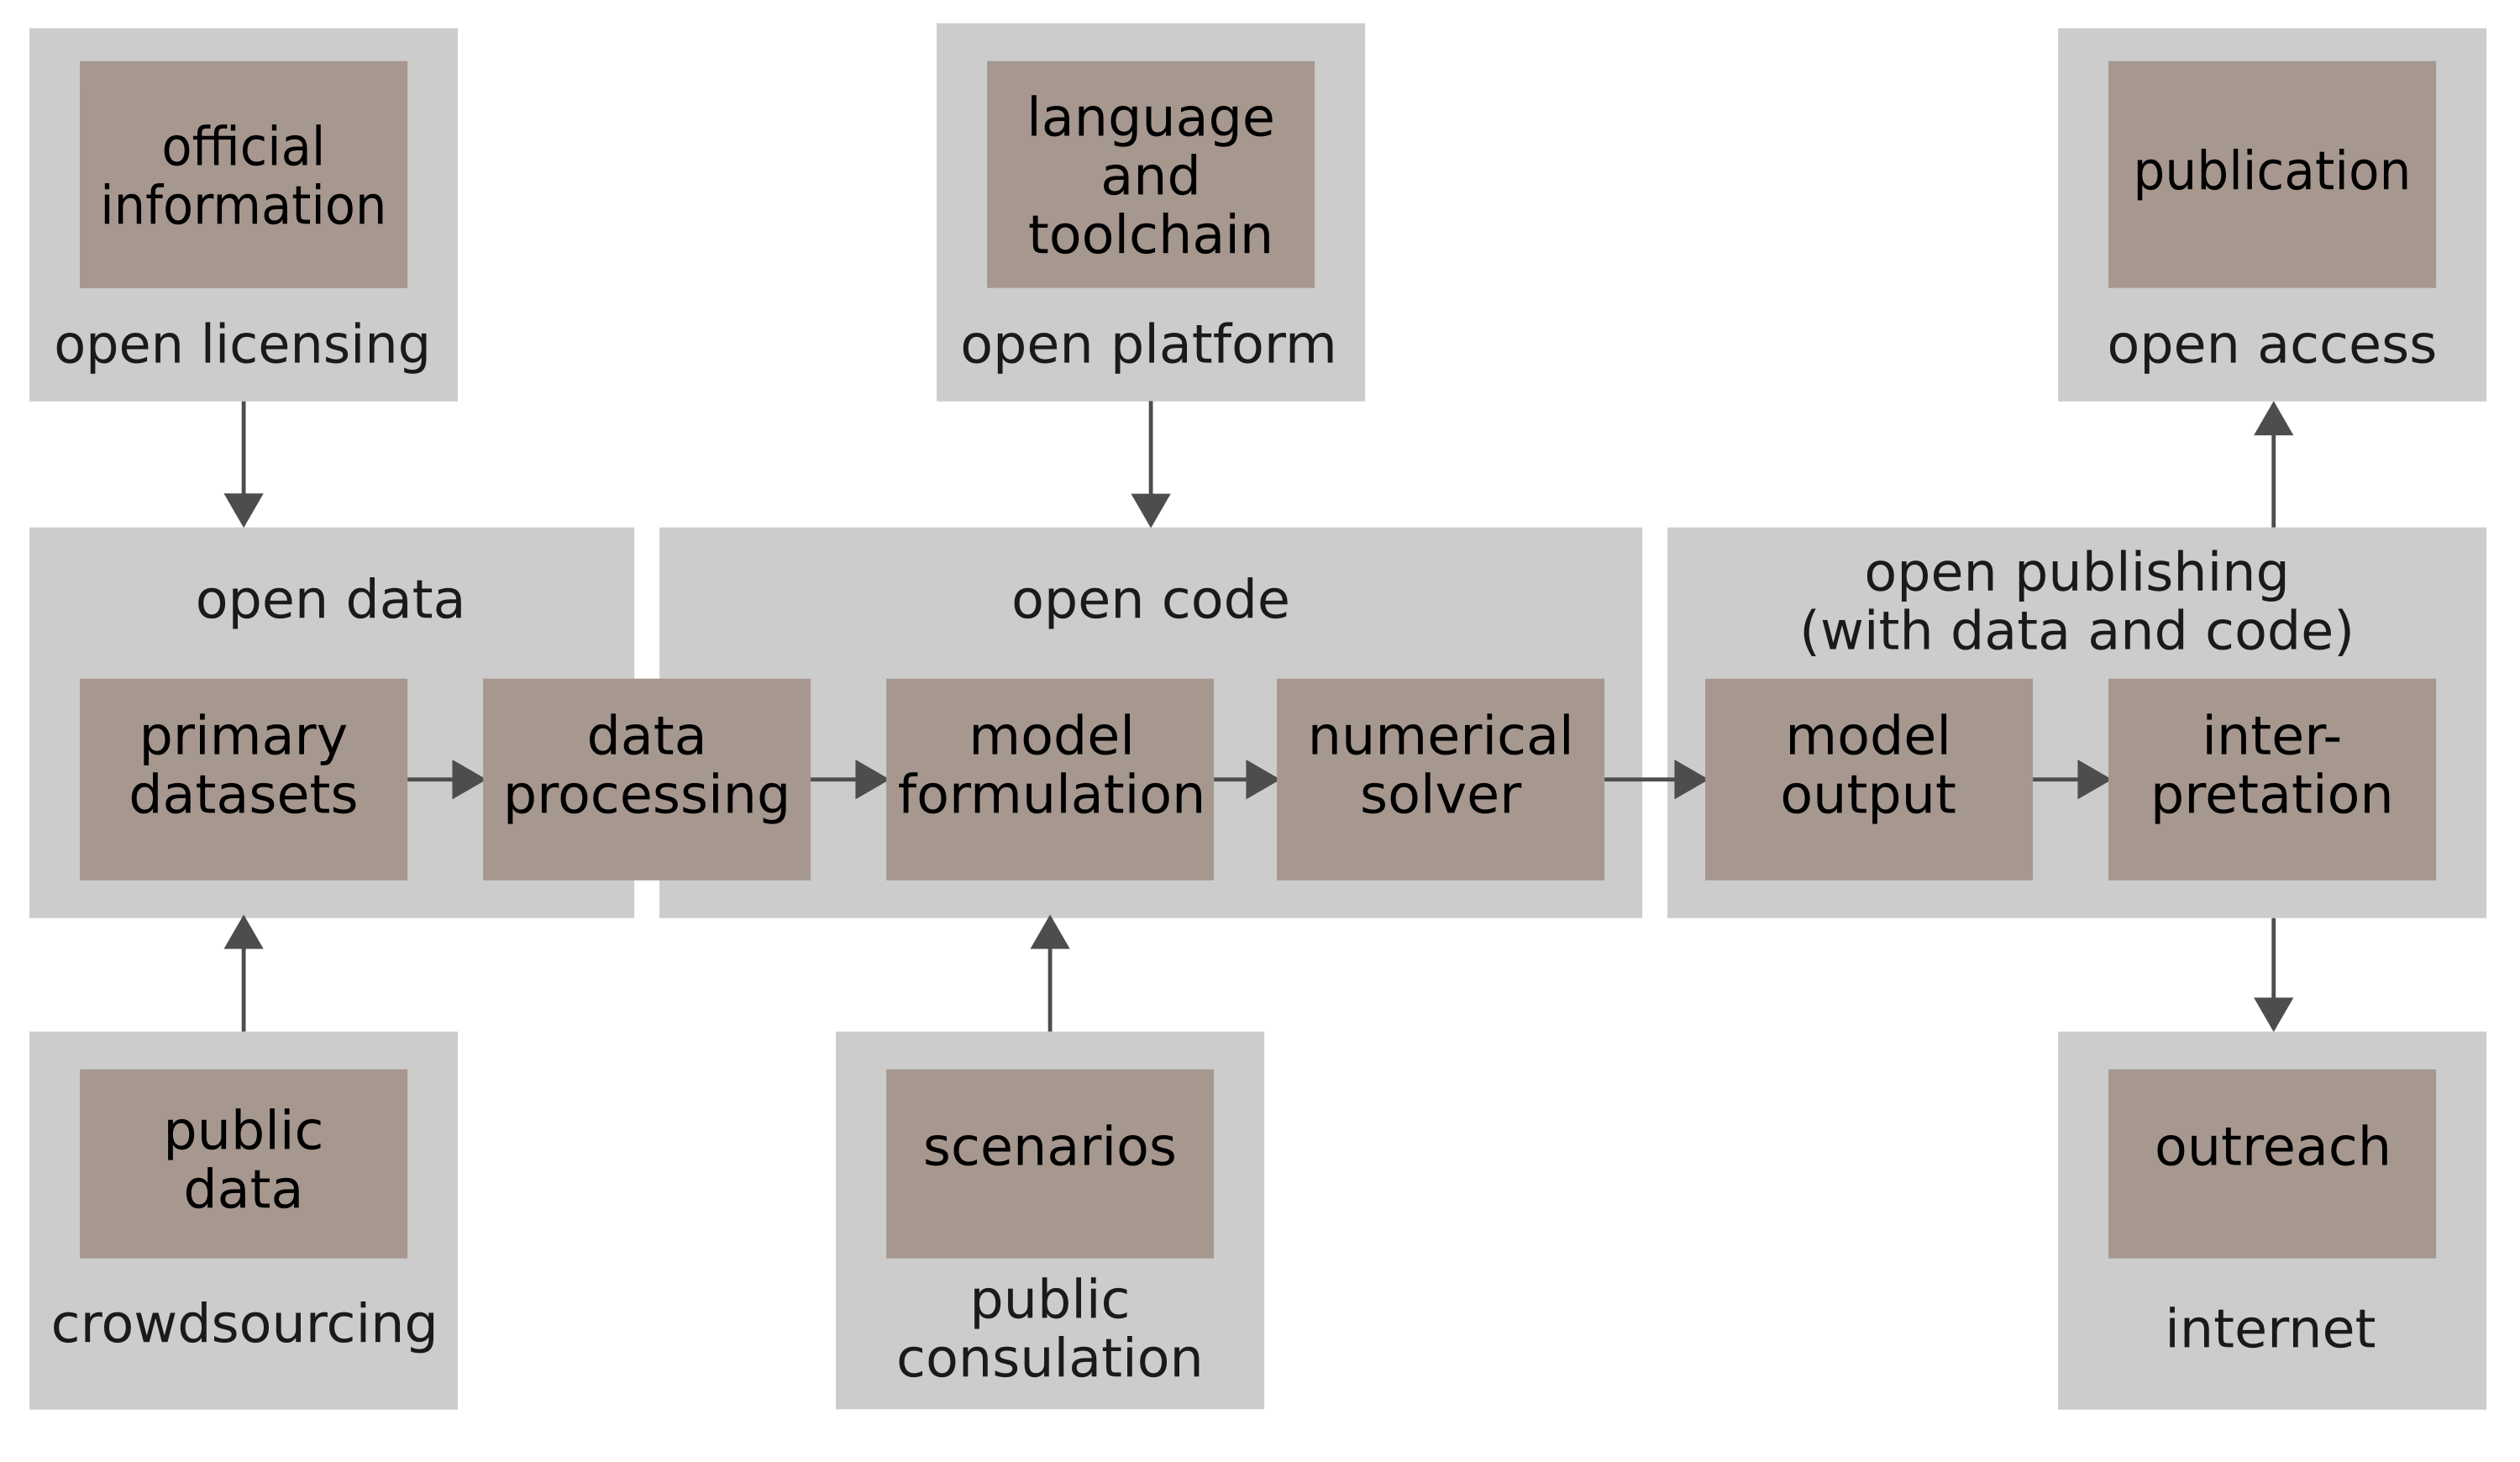
\includegraphics[width=10cm]{open-modeling-chain}

  \source{Robbie Morrison, Eva Schmid, CC 4.0 BY}
\end{frame}


\begin{frame}
  \frametitle{why open modelling?}

  openness \dots
  \begin{itemize}
  \item \dots increases \alert{transparency}, \alert{reproducibility}
    and \alert{credibility}, which lead to better research and policy
    advice  (no more `black boxes')
  \item \dots \emph{can} improve research \alert{quality}
  \item  \dots reduces
    \alert{duplication of effort} and frees time  to develop
    \alert{new ideas}
  \item \dots allows easier \alert{collaboration}
  \item \dots is essential given increasing \alert{complexity} of the energy system
  \end{itemize}
  \end{frame}




\begin{frame}
  \frametitle{what open models are there?}

  Since 2001: zero to {\bf +48} projects and more coming

  {\bf Electricity and energy system models:}
  \begin{itemize}
  \item first wave ({\bf 3}): 2001 balmoral, 2004 deeco, 2005 GnuAE
  \item second wave ({\bf +3}): 2010 OSeMOSYS, 2012 TEMOA, NEMO
   \item  as of 2017 ({\bf +25}): Calliope, CREST, DESSTinEE, DIETER, Dispa-SET, Einstein,
  EMLab-Generation, EMMA, Energy Transition Model, EnergyPATHWAYS,
  ETEM, ficus, GENESYS, NEMO, oemof, OnSSET, pandapower, PowerMatcher,
  PyPSA, renpass, SIREN, StELMOD, SWITCH, URBS, WWS project
  \end{itemize}
\end{frame}

\begin{frame}
  \frametitle{what open models are there?}

  {\bf Transmission and distribution grid models:}
  \begin{itemize}
    \item as of 2017 ({\bf 8}): DINGO, GridKit, GridLAB-D, Hutcheon and Bialek dataset,
  OpenDSS, OpenGridMap, osmTGmod, SciGRID
  \end{itemize}

  {\bf Energy database projects:}
  \begin{itemize}
  \item first wave ({\bf 4}): 2004 OpenStreetMap, 2009 OpenEI, 2011 Enipedia, 2011 reegle
  \item as of 2017 ({\bf +6}): Energy Research Data Portal for South Africa, energydata.info,
  oedb, Open Power System Data, OpenGridMap, Renewables.ninja
  \end{itemize}

\end{frame}


\begin{frame}
  \frametitle{what is the openmod initiative?}

  The openmod initiative consists of a public \alert{\href{https://groups.google.com/forum/\#!forum/openmod-initiative}{mailing list}} (300+ participants) \dots

  \centering
  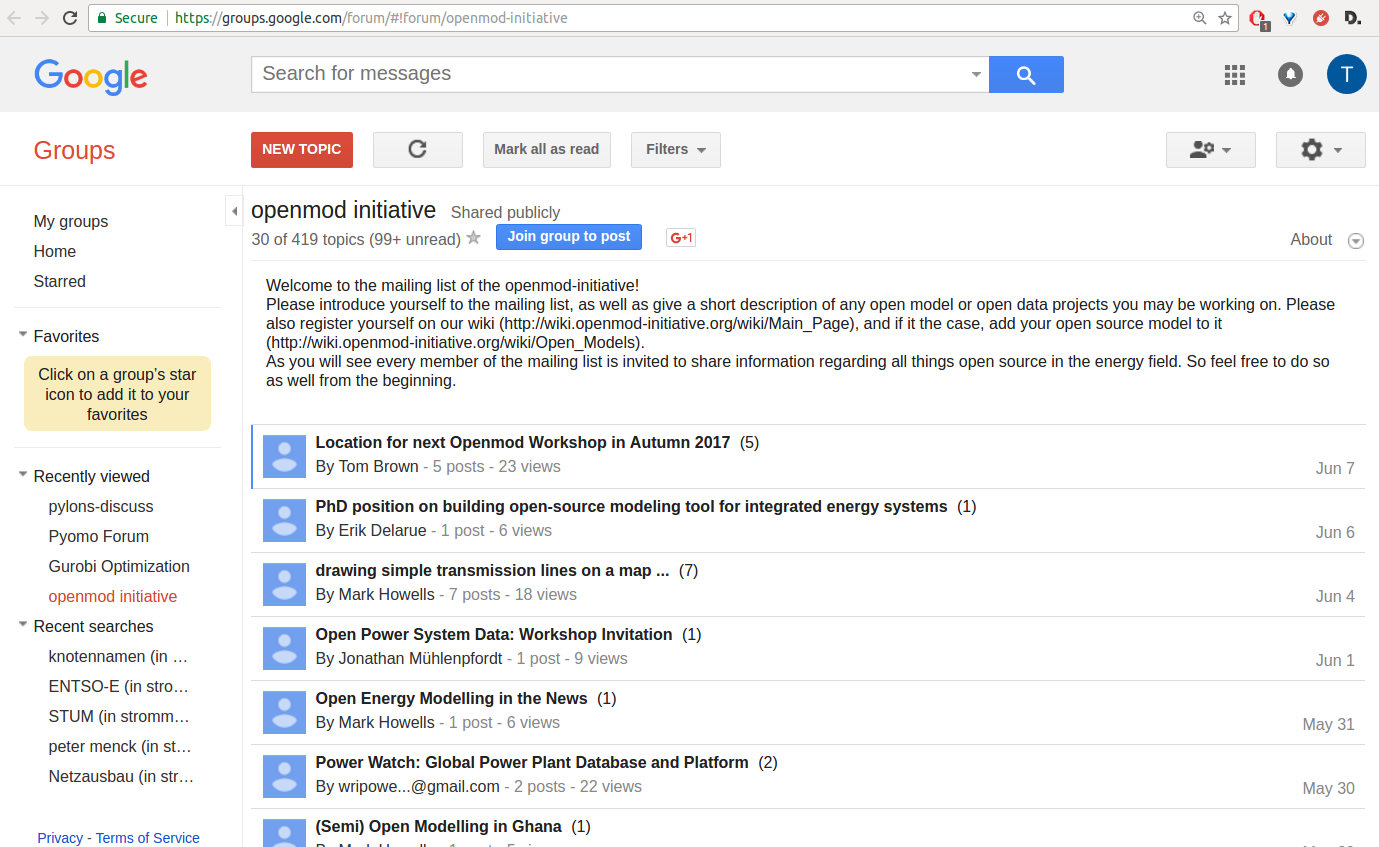
\includegraphics[width=12cm]{openmod-mailing_list}

\end{frame}

\begin{frame}
  \frametitle{what is the openmod initiative?}

  \dots an internet \alert{\href{https://forum.openmod-initiative.org/}{forum}} for more intense discussions, Q \& A and planning \dots

  \centering
  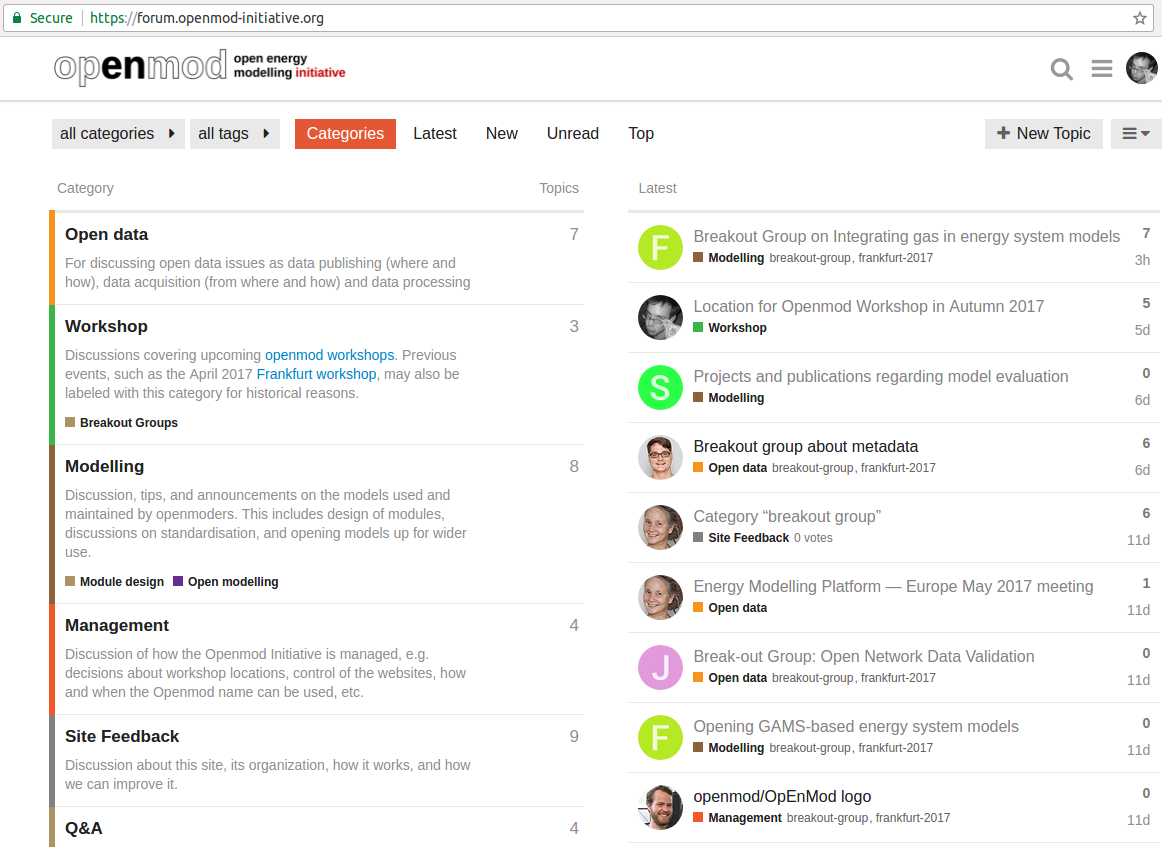
\includegraphics[width=12cm]{openmod-forum}

\end{frame}


\begin{frame}
  \frametitle{what is the openmod initiative?}

  \dots a collaborative \alert{\href{https://wiki.openmod-initiative.org/}{wiki}} for collecting information on models and data \dots

  \centering
  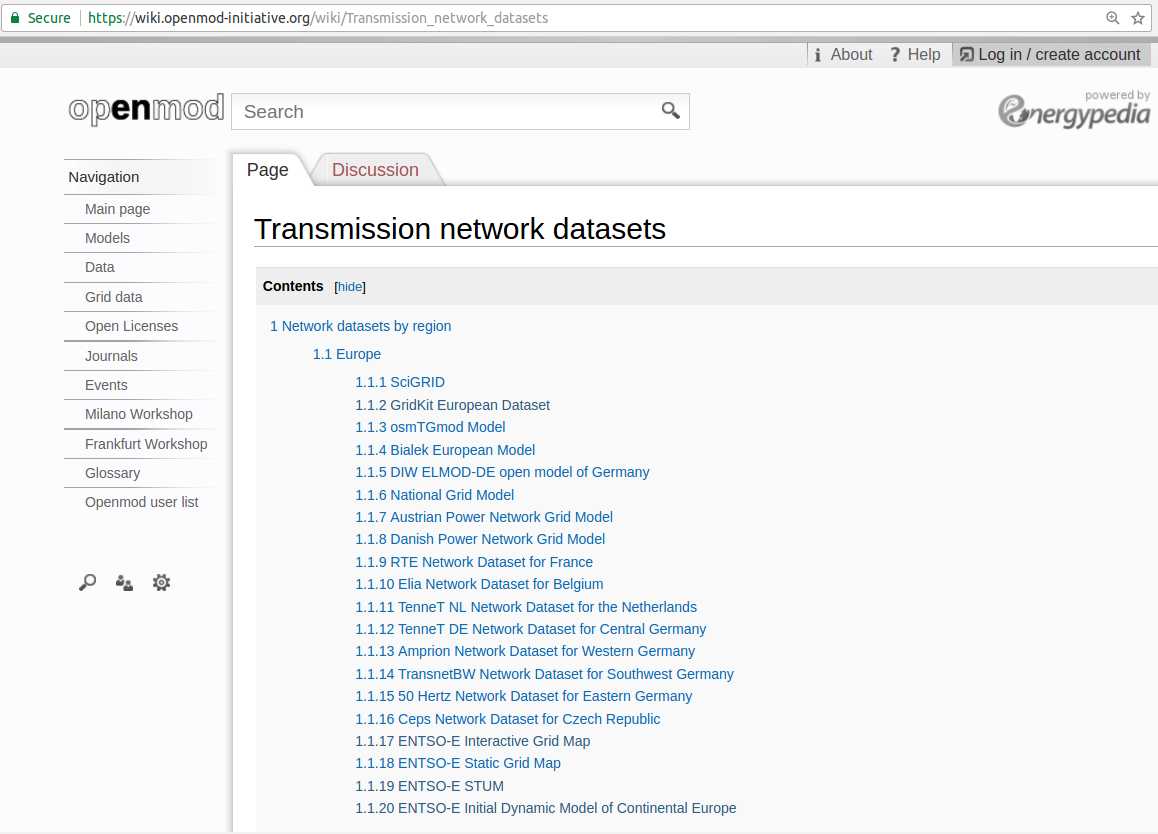
\includegraphics[width=12cm]{openmod-wiki}

\end{frame}

\begin{frame}
  \frametitle{what is the openmod initiative?}

  \dots and finally a \alert{\href{https://wiki.openmod-initiative.org/wiki/Open_Energy_Modelling_Workshop_-_Munich_2017}{workshop}} every six months for two-three days.

  \vspace{.5cm}

  Next Workshop: Technical University of Munich, 11th - 13th October 2017

  \begin{itemize}
  \item  tutorials on open software tools and open energy models
  \item open model and open data presentations
  \item breakout  groups on every possible topic
  \end{itemize}

\end{frame}


\begin{frame}
  \frametitle{what is the openmod initiative currently doing?}

  The following \alert{issues} are currently being tackled by
  openmod members:
  \begin{itemize}
  \item   good practice in open source projects
  \item barriers to developing open source projects
  \item helping data owners understand the consequences of openness
  \item energy data and metadata standards
  \item energy model classification and cataloguing
  \item open/free/libre software and data licensing
  \item    better research computing skills
  \end{itemize}
\end{frame}

\begin{frame}
  \frametitle{want to join the openmod initiative?}

  There is no application process or membership fee. Simply \dots
  \begin{itemize}
  \item \dots join the \alert{\href{https://groups.google.com/forum/\#!forum/openmod-initiative}{mailing list}}
  \item \dots join the online \alert{\href{https://forum.openmod-initiative.org/}{forum}}
  \item \dots check out the \alert{\href{http://openmod-initiative.org/}{website}}
  \item \dots come to the next \alert{\href{https://wiki.openmod-initiative.org/wiki/Open_Energy_Modelling_Workshop_-_Munich_2017}{workshop}}: 11th-13th October 2017,
    Technical University of Munich
  \end{itemize}

\end{frame}
\begin{frame}{Copyright}


  Unless otherwise stated, the graphics and text are Copyright \copyright Tom Brown, Robbie Morrison, 2017.

  The graphics and text for which no other attribution are given are licensed under a
  \href{http://creativecommons.org/licenses/by/4.0/}{Creative Commons
  Attribution 4.0 International Licence}.

  \begin{center}\ccby\end{center}

\end{frame}

\end{document}
